\section{Architecture}

A discussion and a design on the importance of good architecture must take place to comply with the non-functional requirement of the architecture.
A good software design is essential to keep the software's code understandable, simple to extend, and easy to manage.
That applies to the structure of all parts of the software.
\textcquote{martin_2018_clean_architecture}{Software has two types of value: the~value of its behavior and the~value of its structure.
The~second of these is the~greater of the~two because it is this value that makes software soft.}
As mentioned in the cited text, the issue of software is not making its behavior correct and making it work as expected.
The issues developers can face are caused by the poor design of individual parts of the software and its whole.
It's a matter of quality, not quantity.

Many developers tend to write code fast.
They can even think that if the code works, everything is fine.
That might be a truth, but \textcquote{martin_2010_clean_code}{It is not enough for code to work.}
The same functionality can be written in different ways and with various qualities.
No matter how the code was written, it has to be flexible and easy to understand enough so developers can read it and refactor it easily.
Stated and all related reasons combined make software either good or terrible.

What is why developers forced themselves to write working software but with horrible designs?
Maybe companies that try to save money or release as fast as possible?
The actual reason behind that does not matter.
Writing a flexible, easily extendable, and easy-to-read code is not more complex than not doing that.
\textcquote{martin_2010_clean_code}{Indeed, the ratio of time spent reading versus writing is well over 10 to 1.
We are constantly reading old code as part of the effort to write new code. \dots{}
[Therefore,] making it easy to read makes it easier to write.}

The code developers write really should be flexible to changes.
And the same applies to the design.
There is no reasoning behind not making it flexible.
Sticking to designing and coding too specifically might seem to work out at the moment, but changes in the future will be near impossible to make.
The same also applies to extending features or adding new ones.
\textcquote{gamma_1994_design}{A design that doesn't take change into account risks major redesign in the future.}
And many might argue that every code might be improved, and postponing writing flexible code instead of that write code that 'just works' is no big deal.
\textcquote{martin_2010_clean_code}{Of course bad code can be cleaned up.
But it's very expensive.}
Developers should instead use their time to design, build, and code, not to fix issues they could have avoided in the first place.
\textcquote{martin_2018_clean_architecture}{The only way to go fast, is to go well.}

Even if developers agree that individual parts of the code should be written well, flexible, and easy to read and extend, why should they invest in making a good design and architecture?
Because the same issues that have been discussed in the scope of individual parts of code also similarly apply to higher levels.
Choosing the way of easy solutions now instead of proper design brings the software into technical debt. 
\textcquote{martin_2018_clean_architecture}{Good architecture makes the~system easy to~understand, easy to~develop, easy to~maintain, and~easy to~deploy.
The~ultimate goal is to~minimize the~lifetime cost of~the~system
and~to~maximize programmer productivity.}

\subsection{Client-Server Architecture Design}

Multiple options should be considered to design the best approach to create the desired product.
There might be one program that handles everything, or multiple programs, that each does separate tasks.
The software is often separated into the server and client parts, no matter the target platform.
Analyzed requirements also require cross-platformness, as stated in non-functional requirements.
Because of that, cross-platformness almost forces the architecture to divide the software into multiple parts.
The software can be delivered as individual programs to each targeted platform.
Also, a shared functionality can be extracted into a separate part.
The question is how many parts the software should contain to offer the best value and be the easiest to develop.

The standard way of doing such software is to divide the software into two parts: client and server.
A client part mainly handles the aspect of displaying UI (user interface) to users.
Client application usually runs on the user's device and relies on the other part to perform or check some operations.
And a server part that handles incoming requests and processes them.
The server application also usually handles communication with a database.
A database part can also be considered a third part of the software division.
For the software to be cross-platformn, the software contains multiple client implementations, each for a different targeted platform.
This way, the software can have a client for web, desktop, and mobile where all of these clients communicate with the same server application.
That is very economical and also provides the integrity of offered functionalities.

There are many ways in which client applications can be implemented.
Implementations strategies can also be divided into two types.
There are thick clients and thin clients.
Both of them provide benefits and disadvantages, and it is up to the software designer to determine which type would fit the current case the most.
The difference between them is who processes the work, a client or a server?

Thin clients are designed to be small.
They usually process only the data they have to, sending all extra data to a server to process.
That might make thin clients easy to install, as they are usually smaller.
The benefits of this approach might be that a client application can be run almost anywhere, no matter the hardware specifications, because the thin client only displays the data, and the actual processing and work happen in a server application.
The disadvantages are that users often must rely on their internet connection, as most servers are in a different network.

Thick clients are designed to be self-sufficient.
They usually use a server application only as a middleware that handles storing and fetching data to the database.  
Thick clients handle and process most of the data inside of the client.
The benefits of this approach are that even if the client application lost an internet connection or did not have one at all at the moment, the application is still able to do its work, and the data can be stored, synced, or verified later when the internet connection is restored.
The disadvantage that thick clients might face is that all versions of clients must implement all the features that force developers to reinvent the wheel.

Both thick and thin clients provide a lot of benefits and disadvantages.
Therefore a lot of the time, some hybrid clients are used instead.
They combine those two approaches, making most of the processing on the server, especially if that is data-related, and making most of the UI-related processing in the client application.

The designed game should implement a hybrid-like type of client because it uses features of both approaches.
Its data must be stored in servers, but a slow internet will suffice, yet it cannot work without it.
The client part should process all UI-related functionality and game-related processing, but the server should handle the data storing, data processing and verifying, and authentication.

\subsection{Selection of Architectures for Client and Server}

As software development evolved and improved, new ways of designing and new architectures appeared and tried a battle against time.
As mentioned in~\cite{a2021_clean_architecture_blog}, many architectures of systems try to achieve similar goals.
The most common primary goal of architectures is to address the separation of concerns.
Architectures like Hexagonal Architecture, Onion Architecture, and Clean Architecture separate concerns into different software layers.
Such architectures and their layers should be independent of UI, frameworks, databases, or other external tools.
If architecture depends on one of those things, it would significantly limit its abilities, which is not desirable.
Architecture should be generic and should not compromise with specific tools.

The article~\cite{a2021_clean_architecture_blog} also mentiones the dependency rule.
This rule describes requirements for a flow of software layers.
Outer layers do specific things and use inner layers that describe policies.
Therefore, the dependencies should always come from an outer layer to an inner layer.
Inner layers should not even know some outer layer exists.
This rule applies to all the code inside the layer, whether a class, a function, or any other entity.
The inner layer commonly contains business rules like entities and use cases.
Outer layers commonly contain layers with interface adapters and frameworks.
The number of layers can vary from architecture to architecture.
The important thing is the concept: the separation of details and abstractions and that only details can point to abstractions, not the other way around.
Architectures also must solve how to cross the boundaries of layers and call abstractions that have to use details.
That is typically done by using the dependency inversion principle described in~\ref{design:architecture:clean-archiecture}.

Both the client and the server parts should use a good architecture that uses mentioned concepts.
The goals are the same: to create flexible and manageable codebases.
Both parts will use architectures similar to the Clean Architecture, especially its dependency inversion principle and other SOLID principles.
\textcquote{martin_2018_clean_architecture}{Good software systems begin with clean code.
On~the~one hand, if the~bricks aren't well made, the~architecture of~the~building doesn't matter much.
On~the~other hand, you can make a~substantial mess with well-made bricks.
This is where the~SOLID principles come in.}

\subsection{The Clean Architecture}
\label{design:architecture:clean-archiecture}

The~Clean Architecture was described in an~eponymous book~\cite{martin_2018_clean_architecture} authored by Robert~C. Martin, also known by the nickname Uncle Bob.
The author is an American software engineer known for the invention or promotion of~software principles, especially the SOLID principles.

\begin{figure}
    \centering
    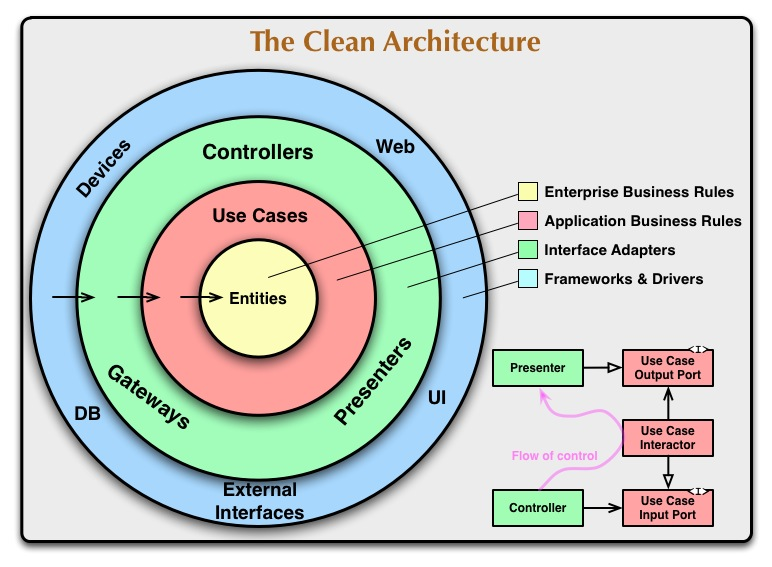
\includegraphics[width=1\linewidth]{assets/design/cleanarchitecture.jpg}
    \caption{The Clean Architecture}
    \label{fig:thecleanarchitecture}
\end{figure}

The book~\cite{martin_2018_clean_architecture} explains multiple topics.
It discusses paradigms of programming: benefits and disadvantages of structured programming, object-oriented programming, and functional programming.
There is a discussion about what these paradigms remove from developers, like assignments, goto statements, pointers, etc.
The section about object-oriented programming brings a dependency inversion, allowing dependency to point in the inverted direction compared to the flow of control.
The dependency inversion principle is a pillar of The Clean Architecture, alongside the single responsibility principle.
The single responsibility principle states that every module should have only one reason to change, and therefore, that module should be responsible to only one actor.

There are more SOLID principles.
The open-closed principle describes how entities should be open for an extension rather than change.
The Liskov substitution principle explains that extensions should be substitutable for their origin.
And interface segregation principle that explains that implementation of things that are not used should be avoided.

\begin{description}
    \item[Single-responsibility principle] \textcquote[p.~57--59]{martin_2018_clean_architecture}{An active corollary to 
Conway's law:\linebreak
The~best structure for a~software system is heavily influenced
by the~social structure of the~organization that uses it so that
each software module has one, and only one, reason to change.}
    \item[Open--closed principle] \textcquote[p.~57--59]{martin_2018_clean_architecture}{Bertrand Meyer made this principle famous\linebreak in~the~1980s.
The gist is that for software systems to be easy to change,
they must be designed to allow the behavior of those systems to be changed by~adding new code, rather than changing existing code.}
    \item[Liskov substitution principle] \textcquote[p.~57--59]{martin_2018_clean_architecture}{Barbara Liskov's famous definition of subtypes, from~1988.
    In short, this principle says that to build software systems from interchangeable parts, those parts must adhere to a~contract that allows those parts to be substituted one for another.}
    \item[Interface segregation principle] \textcquote[p.~57--59]{martin_2018_clean_architecture}{This principle advises
software designers to avoid depending on things that they don't use.}
    \item[Dependency inversion principle] \textcquote[p.~57--59]{martin_2018_clean_architecture}{The code that implements high-level policy should not depend on the code that implements low-level details.
Rather, details should depend on policies.}
\end{description}
